%!TEX root=writeup.tex
\section{Evaluation}
\label{sec:eval}
To evaluate the effectiveness of our tool in verfication of SQL rewrting rules, we collect 6 different types of SQL rewriting rules as our testing benchmark and evalute our tool on these 6 examples. And our evaluation goal is to answer the following three research quesionts.
\begin{itemize}\itemsep0pt
\item Whether our prototype can verify the correctness of rewriting rules.
\item Whether our prototype can find erros in wrong rewrting rules.
\item How does our prototype scale with the size of the symbolic input tables.
\end{itemize}

\paragraph{Proving Rewriting Rules on Bounded schema}
Code Snippet XXX shows one of our rewriting rules. 
SQL query equivalence with such level of complexity may be hard for a human being to 
figure out, but the verifier can verify the equivalence of queries on a bounded-sized 
schema within a reasnable amount of time.

\begin{figure}
\begin{lstlisting}[style=sql]
SELECT DINSTINCT a, b
FROM R
\end{lstlisting}
\caption{Magic Set Rewrite}
\end{figure}

\paragraph{Detecting Incorrect Rewriting Rules}
Code Snippet XXX is an example of an incorrect SQL rewriting rule.
When running these two SQL queries on our verifier, a counterexample will be returned that
shows in which case the two queries are not equivalent.
This functionality can be potentially useful for SQL query optimization validation.

\paragraph{Scalability}
To illustrate the scalability of our prototype implementation, we evaluated
6 rewriting rules with different symbolic schema sizes on a desktop PC
~\footnote{The PC has 3.60GHz Intel Core i7 CPU, and 8 GB of memeory}.
Figure~\ref{fig:scale} shows the time it takes to verify the equivalence of SQL queries
with different symbolic schema sizes.

\begin{figure}[!htb]
  \centering
  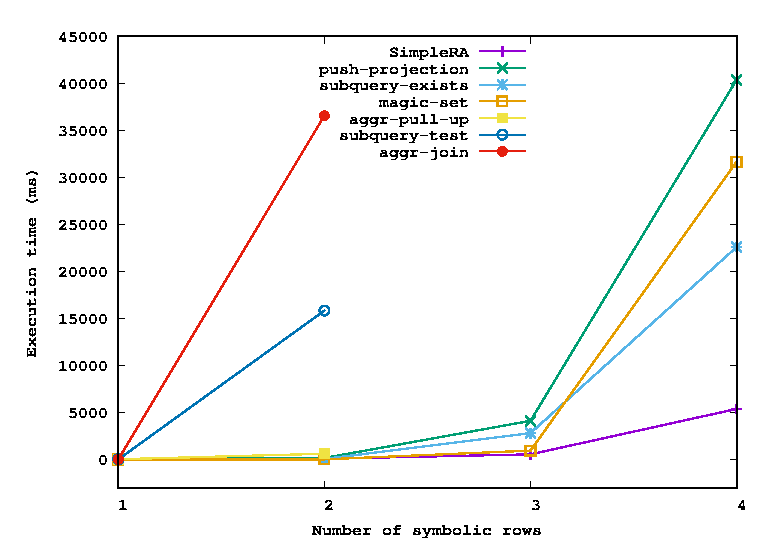
\includegraphics[width=0.7\linewidth]{scale.eps}
  \caption{\# of Symbolic Rows v. Verification Execution Time}
  \label{fig:scale}
\end{figure}

From the figure, we can see that the scalability of the verifier heavily depends 
on the complexity of the rewriting rules.
For those rewriting rules without table join and subquery, it can scales pretty well.
For rewriting rules with either table join or subquery, the prototype implementation can 
not scale well with the growing of the size of the symbolic schema.
Based on our evaluation, queries with both table join and subquery can not scale to schema with
more than 2 rows.

%%% Local Variables:
%%% mode: latex
%%% TeX-master: "writeup"
%%% End:
